\begin{frame}{Luồng đăng ký và kiểm tra xác thực MFA với Supabase}
\begin{figure}[H]
\centering
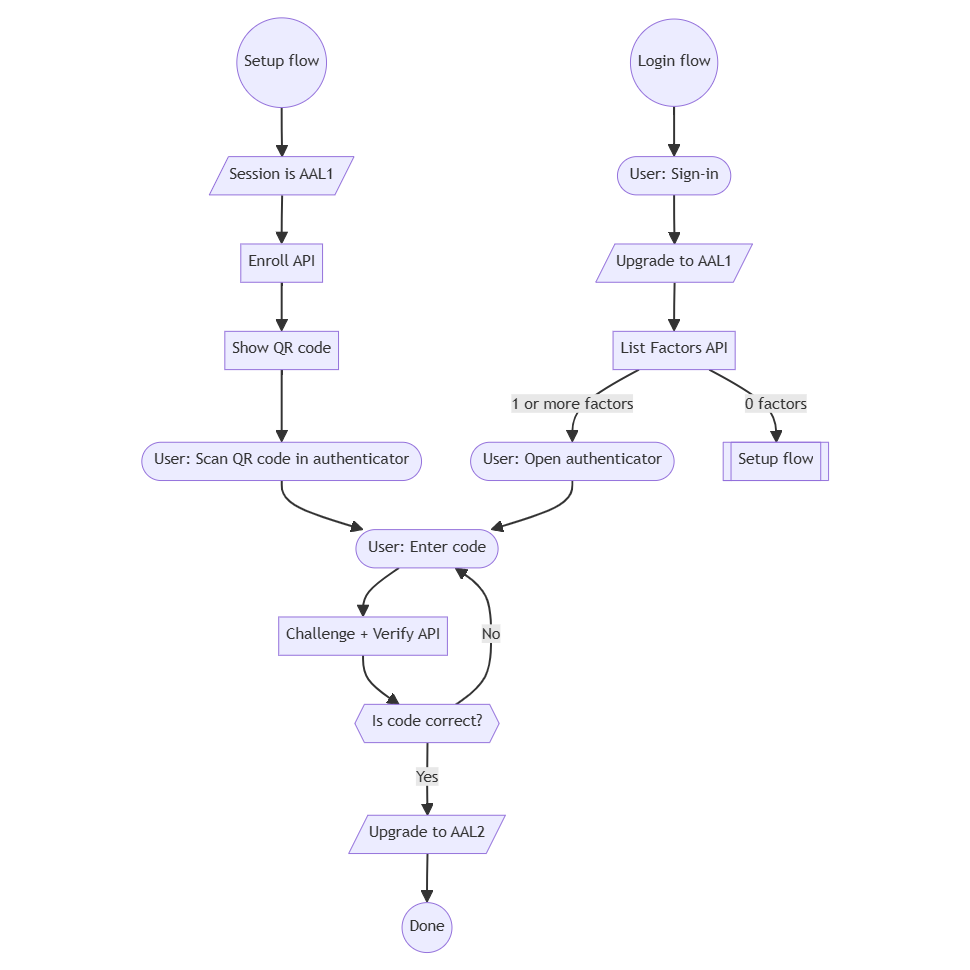
\includegraphics[height=0.55\textheight,width=0.9\textwidth,keepaspectratio]{pictures/auth-mfa-flow.excalidraw.png}

\caption[Sơ đồ luồng xử lý xác thực MFA Supabase]{Sơ đồ luồng xử lý xác thực MFA Supabase (Nguồn: \footnotemark)}
\end{figure}
\footnotetext{\url{https://supabase.com/docs/guides/auth/auth-mfa/totp}}

\note{
Sơ đồ mô tả quy trình đăng ký (Enrollment) và quy trình kiểm tra đăng nhập (Challenge) của tính năng MFA tích hợp với Supabase.
Khi người dùng đăng nhập lần đầu, họ ở cấp độ bảo mật aal1. Hệ thống sẽ trích xuất danh sách các yếu tố MFA đã đăng ký, gọi hàm challenge để tạo phiên thử thách và sau khi người dùng nhập đúng mã TOTP, gọi hàm verify để hoàn tất và nâng cấp cấp độ phiên làm việc lên aal2.
}
\end{frame}
